\documentclass[a4paper, 12pt]{article}
\usepackage[utf8]{inputenc}
\usepackage{fullpage}
\usepackage[italian]{babel}
\usepackage{parskip}
\usepackage{setspace}
\usepackage{hyperref}
\usepackage{biblatex}
\usepackage{subfiles}
\usepackage{graphicx}
\usepackage[justification=centering]{caption}% or e.g. [format=hang]
\addbibresource{references.bib}

\hypersetup{
    colorlinks=true,
    linkcolor=black,
    filecolor=magenta,
    urlcolor=cyan,
    pdftitle={Vivere in libertà},
    pdfpagemode=FullScreen,
}

\urlstyle{same}

\title{Lo stato democratico\break
Il valore della vita PDI}
\author{Samuel Banfi, Dennis Donofrio}
\date{}

\begin{document}

\maketitle

\pagebreak

\tableofcontents

\pagebreak

\onehalfspacing

\section{Introduzione}

\subsection{Presentazione}

\subsubsection{Samuel Banfi}

Mi chiamo Samuel Banfi, ho 20 anni e sono al quarto anno presso la scuola d'arti e mestieri a Trevano. Sono nella classe I4AC e le mie passioni sono il montaggio di foto / video e la programmazione. Negli ultimi mesi mi sto interessando al mondo degli investimenti. Quest'ultimo mi è tornato utile per comprendere meglio le situazioni economiche delle nazioni.

\subsubsection{Dennis Donofrio}

Mi chiamo Dennis Donofrio, ho 18 anni e abito a Taverne. Sto frequentando la scuola di informatica presso l'arti e mestieri a Trevano in una piccola classe di 12 persone. Ho scelto di diventare informatico perchè mi è sempre piaciuto il mondo dell'informatica, in tutte le sue sfaccettature. Inoltre mi piace fare foto e video, lavorare con auto e moto e tanto altro. Da quando è scoppiata la guerra in Ucraina mi sono chiesto quale fosse il valore della vita.

\subsection{Descrizione}

Questo lavoro coinvolge le materie di storia ed economia e diritto. I docenti coinvolti in questo lavoro sono Monica Delucchi e Ursula Holliger. L'argomento generale tratta lo stato democratico, mentre l'argomento specifico di cui parliamo noi è "il valore della vita". Abbiamo scelto questo argomento visto l'attuale situazione nella quale ci troviamo. La Russia e l'Ucraina combattono sacrificando la vita dei suoi cittadini, il Qatar invece ha sacrificato la vita di più di 6000 persone solamente per costruire uno stadio.

\pagebreak

\subsection{Domanda di ricerca}

\textbf{Perché le persone si sacrificano per l'obbedienza?} \\\\
Con l'assegnazione dei mondiali di calcio, si è fatto riconoscere per lo sfruttamento dei lavoratori, costretti a turni di tante ore al giorno, più di quelle che potrebbe lavorare una persona. Essi ricevono un salario molto basso usato per ripagare il debito contrattato per lavorare lì. In questo modo non sono liberi, perché sono vincolati dal debito e non possono lasciare liberamente il lavoro. Questa è una tipologia di schiavitù della nostra epoca. \\ Secondo noi non vale la pena perdere la vita per nessun tipo di lavoro. La vita è un dono che non si può comprare e non va buttata via e per questo motivo non vale la pena morire per un lavoro. L'unico motivo per cui qualcuno potrebbe essere disposto a perdere la vita, sarebbe per aiutare la propria famiglia (molto spesso in modo economico) per garantire un futuro più roseo per i figli. Inoltre, lo sfruttamento dei lavoratori non dà la possibilità di vivere una vita dignitosa per sé e per la propria famiglia. In Qatar sono morte più di 6500 persone per la costruzione di stadi e infrastrutture per i mondiali. L'unica cosa che facevano era lavorare, l'unica cosa che ricevevano era cibo. In questo modo la vita non ha più senso. Non puoi goderti dei bei momenti con gli amici o con le persone care. Oltre al fatto di non avere più soldi non hai più neanche tempo e salute per fare quello che vuoi. Ma gli schiavi non sono gli unici a perderci. Anche le nazioni (in questo caso il Qatar) hanno grandi perdite finanziarie. Infatti queste persone, non avendo entrate non possono neanche partecipare alle spese della nazione e di conseguenza ad aiutarla a crescere. Gli unici che ci guadagno sono le persone che sfruttano la mano d'opera.

\pagebreak

\subsection{La democrazia}

La democrazia è un sistema politico basato sulla volontà del popolo. Di conseguenza è il popolo ad avere il potere. Grazie a questo sistema politico non vi è un singolo individuo a gestire lo stato, ma è l'unione delle persone che si impegnano attivamente per dare valore alla vita di tutti. Un vantaggio che si trova esclusivamente nella democrazia è l'uguaglianza tra le persone e la loro libertà.

\begin{itemize}
    \item L'uguaglianza corrisponde al fatto che ognuno è "giudicato" allo stesso modo, ovvero in modo equo. Senza l'uguaglianza di giudizio qualcuno potrebbe comportarsi in modo scorretto nei confronti di qualcun' altro e non essere punito in modo equo.
    \item La libertà corrisponde al potersi gestire autonomamente senza avere un "capo" che ti costringe a fare qualcosa. Chiaramente entro i limiti della legge.
\end{itemize}

Grazie alla democrazia le persone sono libere di ragionare con la propria testa e non sono limitate ad esempio nella possibilità di informarsi. Purtroppo, in molti stati non vi è ancora la possibilità di votare usando la propria testa, perché c'è una dittatura o semplicemente perché non è stata data un'istruzione uguale a tutti. Se un cittadino non ha la possibilità di informarsi, se le informazioni che gli vengono date sono alterate, egli non sa come comportarsi e si ritrova a votare come tutti gli altri o come "consigliano" i media (social media inclusi). Senza la democrazia i cittadini vengono controllati da una persona o da un gruppo ristretto. Il problema in questi stati sta nel fatto che non vi è una separazione dei poteri. Il potere legislativo, il potere esecutivo e il potere giudiziario sono tutti nelle mani di una sola persona. In questi casi non c'è una vera legislazione e le leggi sarebbero fatte esclusivamente a favore della persona a direzione dello stato perché può decidere cosa punire o meno (leggi).

\subsection{L'importanza della libertà di espressione}

Per libertà di espressione si intende che ogni persona ha il diritto di dire quello che pensa. Questa libertà avvolte è dettata dalle leggi che ne limitano la divulgazione di alcuni temi particolari. La libertà di espressione include la libertà di opinione e la libertà di divulgare informazioni. Questa viene garantita dalle leggi. Negli stati dove la libertà di espressione è limitata possono esserci anche delle conseguenze drammatiche per quanto riguarda la vita della persona che decide di esercitare queste libertà. In alcuni stati se si scrive un articolo contro la persona al potere si rischia la morte (casi di omicidi irrisolti).

\pagebreak

\section{La Russia}

\subsection{La situazione politica}

La Russia oggi è uno degli stati che limita di più la libertà dei cittadini e dei media locali. L'ascesa al potere di Vladimir Putin nel 2000 è stata fatta in modo democratico. In realtà la prima elezione di Putin è stata fatta direttamente dal presidente Eltsin prima di dimettersi. Nel 2004 è stato rieletto e ha ottenuto ancora più consensi dopo essere salito al potere vendicandosi contro la Cecenia. Putin ha ottenuto la possibilità di rimanere al potere oltre al suo quarto mandato grazie ad un voto nazionale sulle riforme costituzionali. Anche la sua immagine di "uomo forte" lo ha reso importante agli occhi dell'opinione pubblica.

% https://www.notiziegeopolitiche.net/russia-lascesa-del-potere-di-putin-dal-1999-ad-oggi/

% https://www.treccani.it/enciclopedia/la-questione-politica-della-russia-contemporanea_%28XXI-Secolo%29/

\subsection{L'economia dello stato Russo}

La Russia è considerata una delle più grandi super-potenze mondiali. I dati dimostrano come nel 2021, il prodotto interno lordo dello stato russo ammontava a 1'439 miliardi di euro. Il PIL di questa nazione era uno tra i più alti al mondo. Negli anni 2022 e 2023 la situazione si è aggravata, infatti con le sanzioni emanate per limitare il conflitto con l'Ucraina, il PIL della Russia scenderà dal 1\% al 4\% tra il 2022 e 2023. Questo molto probabilmente è dovuto anche alla chiusura dei gasdotti Nord Stream 1 e Nord Stream 2 che riforniscono gran parte dell'Europa. I tassi di interesse in Russia sono aumentati tantissimo a causa dell'inflazione, ovvero la nazione si trova senza liquidità. 

\begin{figure}[h]
    \centering
    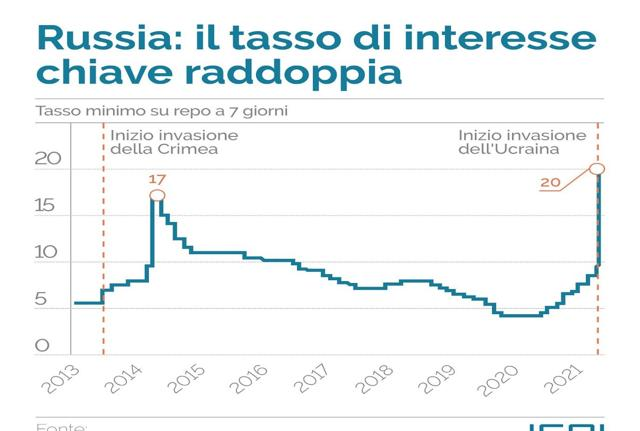
\includegraphics[width=0.75\textwidth]{images/grafico_tassi_interesse_russia.jpeg}
    \caption{Grafico tassi interesse Russia}
\end{figure}

%https://www.startmag.it/mondo/la-russia-e-una-grande-potenza/

%https://www.affaritaliani.it/esteri/sanzioni-russia-impatto-economia-784031.html

\pagebreak

\subsubsection{La libertà di espressione}

In Russia la libertà di espressione, ad esempio la libertà di stampa non viene negata a livello legislativo, viene solamente limitata. Non si può scrivere articoli contro la politica in Russia. Purtroppo per evitare problemi a livello legale i giornalisti hanno applicato l'auto-censura, che consiste nel limitare la divulgazione dei propri pensieri "volontariamente". Secondo una ricerca da quando Vladimir Putin è salito al potere sono stati uccisi 21 giornalisti. Tra gli anni 90 e il 2006, con Putin già al potere, la situazione era molto più grave. Infatti risultano più di 300 giornalisti scomparsi in circostanze sospette. Attualmente, a seguito del conflitto in atto con l'Ucraina (dal 24 febbraio 2022), la libertà di espressione è ancora più limitata. In Russia ci sono state delle proteste per porre fine al conflitto. Per dimostrare l'inesistenza della libertà di espressione ecco un video dove viene mostrata una donna che viene portata via nonostante abbia solamente un cartellone bianco in mano. \href{https://youtube.com/shorts/KzB5-r8un0k?feature=share}{Video}. Come si può notare, la paura delle forze dell'ordine riguardo ad una rivolta popolare, portano a conseguenze drastiche nei confronti dei cittadini. Infatti la donna nel video è stata arrestata nonostante il cartellone fosse bianco, per dimostrare la paura di Vladimir Putin per le rivolte e come fa sopprimere le rivolte in modo alquanto discutibile. A parer mio, vedendo queste scene, i cittadini russi hanno ancora più paura delle conseguenze. Un alto esempio della violazioni dei diritti sulla libertà di stampa lo si può trovare nei giornali russi. Infatti gli abitanti, all'inizio (ma anche ora in parte) del conflitto, dicevano la guerra con l'Ucraina non esisteva.

\begin{figure}[h]
    \centering
    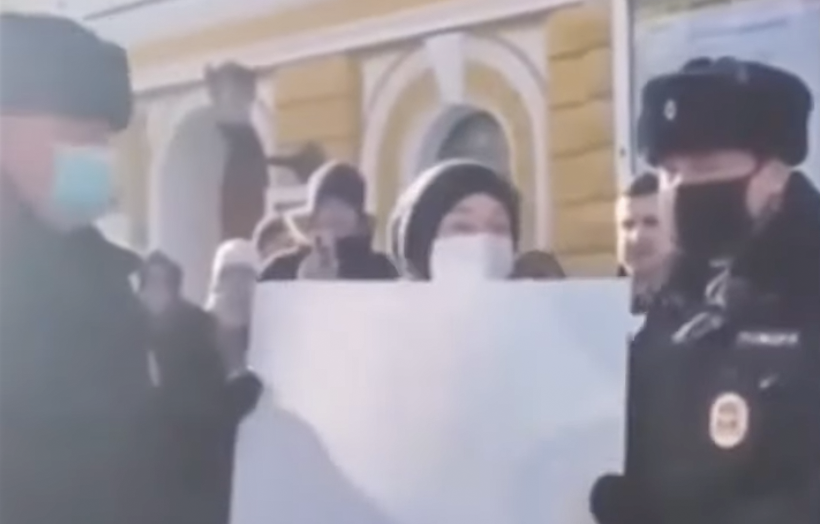
\includegraphics[width=0.75\textwidth]{images/blank_billboard.png}
    \caption{Ragazza arrestata con cartellone vuoto\\\hspace{\textwidth}\href{https://youtube.com/shorts/KzB5-r8un0k?feature=share}{https://youtube.com/shorts/KzB5-r8un0k?feature=share}}
\end{figure}

%https://it.wikipedia.org/wiki/Libert%C3%A0_dei_media_in_Russia

%https://www.treccani.it/vocabolario/autocensura/

%https://it.wikipedia.org/wiki/Giornalisti_uccisi_in_Russia

%https://www.micromega.net/in-piazza-contro-la-guerra-di-putin/

\pagebreak

\subsection{La guerra contro l'Ucraina}

Il 24 febbraio 2022 la Russia ha invaso l'Ucraina, scatenando una guerra che ha portato alla condanna quasi unanime dalla comunità internazionale che ha applicato delle sanzioni contro la Russia.

\subsubsection{Quali sono i motivi del conflitto?}

La Russia è sempre stata d'accordo con l'Ucraina per far si che quest'ultima non entrasse a far parte della NATO (Organizzazione Intergovernativa). Il problema della Russia, se l'Ucraina fosse entrata nella NATO, la Russia si sarebbe ritrovata con tutti i paesi confinanti appartenenti all'organizzazione intergovernativa. Questa guerra viene definita dalla Russia come "operazione speciale", questo sarebbe una scusa per riconquistare dei territori che dovrebbero appartenergli. Uno degli obiettivi militari principali era la conquista del Donbass.

% https://www.rainews.it/articoli/2022/09/allinizio-dellinvasione-vladimir-putin-rigett-un-accordo-di-pace-con-lucraina-fe0bc634-0240-45fc-9c0c-0e2bb4bfc6a3.html

\subsubsection{Il valore del Donbass}

Per la Russia il Donbass non è solamente un obiettivo militare, bensì è anche un obiettivo economico. Con la conquista di quel territorio di ben 51368 km$^2$, la Russia avrebbe la possibilità di sfruttare le sue risorse naturali. Il Donbass è una terra ricca di carbone, gas naturale, uranio, titanio,... Il suo valore economico è estremamente elevato anche perché sono dei materiali rari da trovare oggi (esempio crisi dei semiconduttori dovuta al lockdown e al lavoro da casa).

\begin{figure}[h]
    \centering
    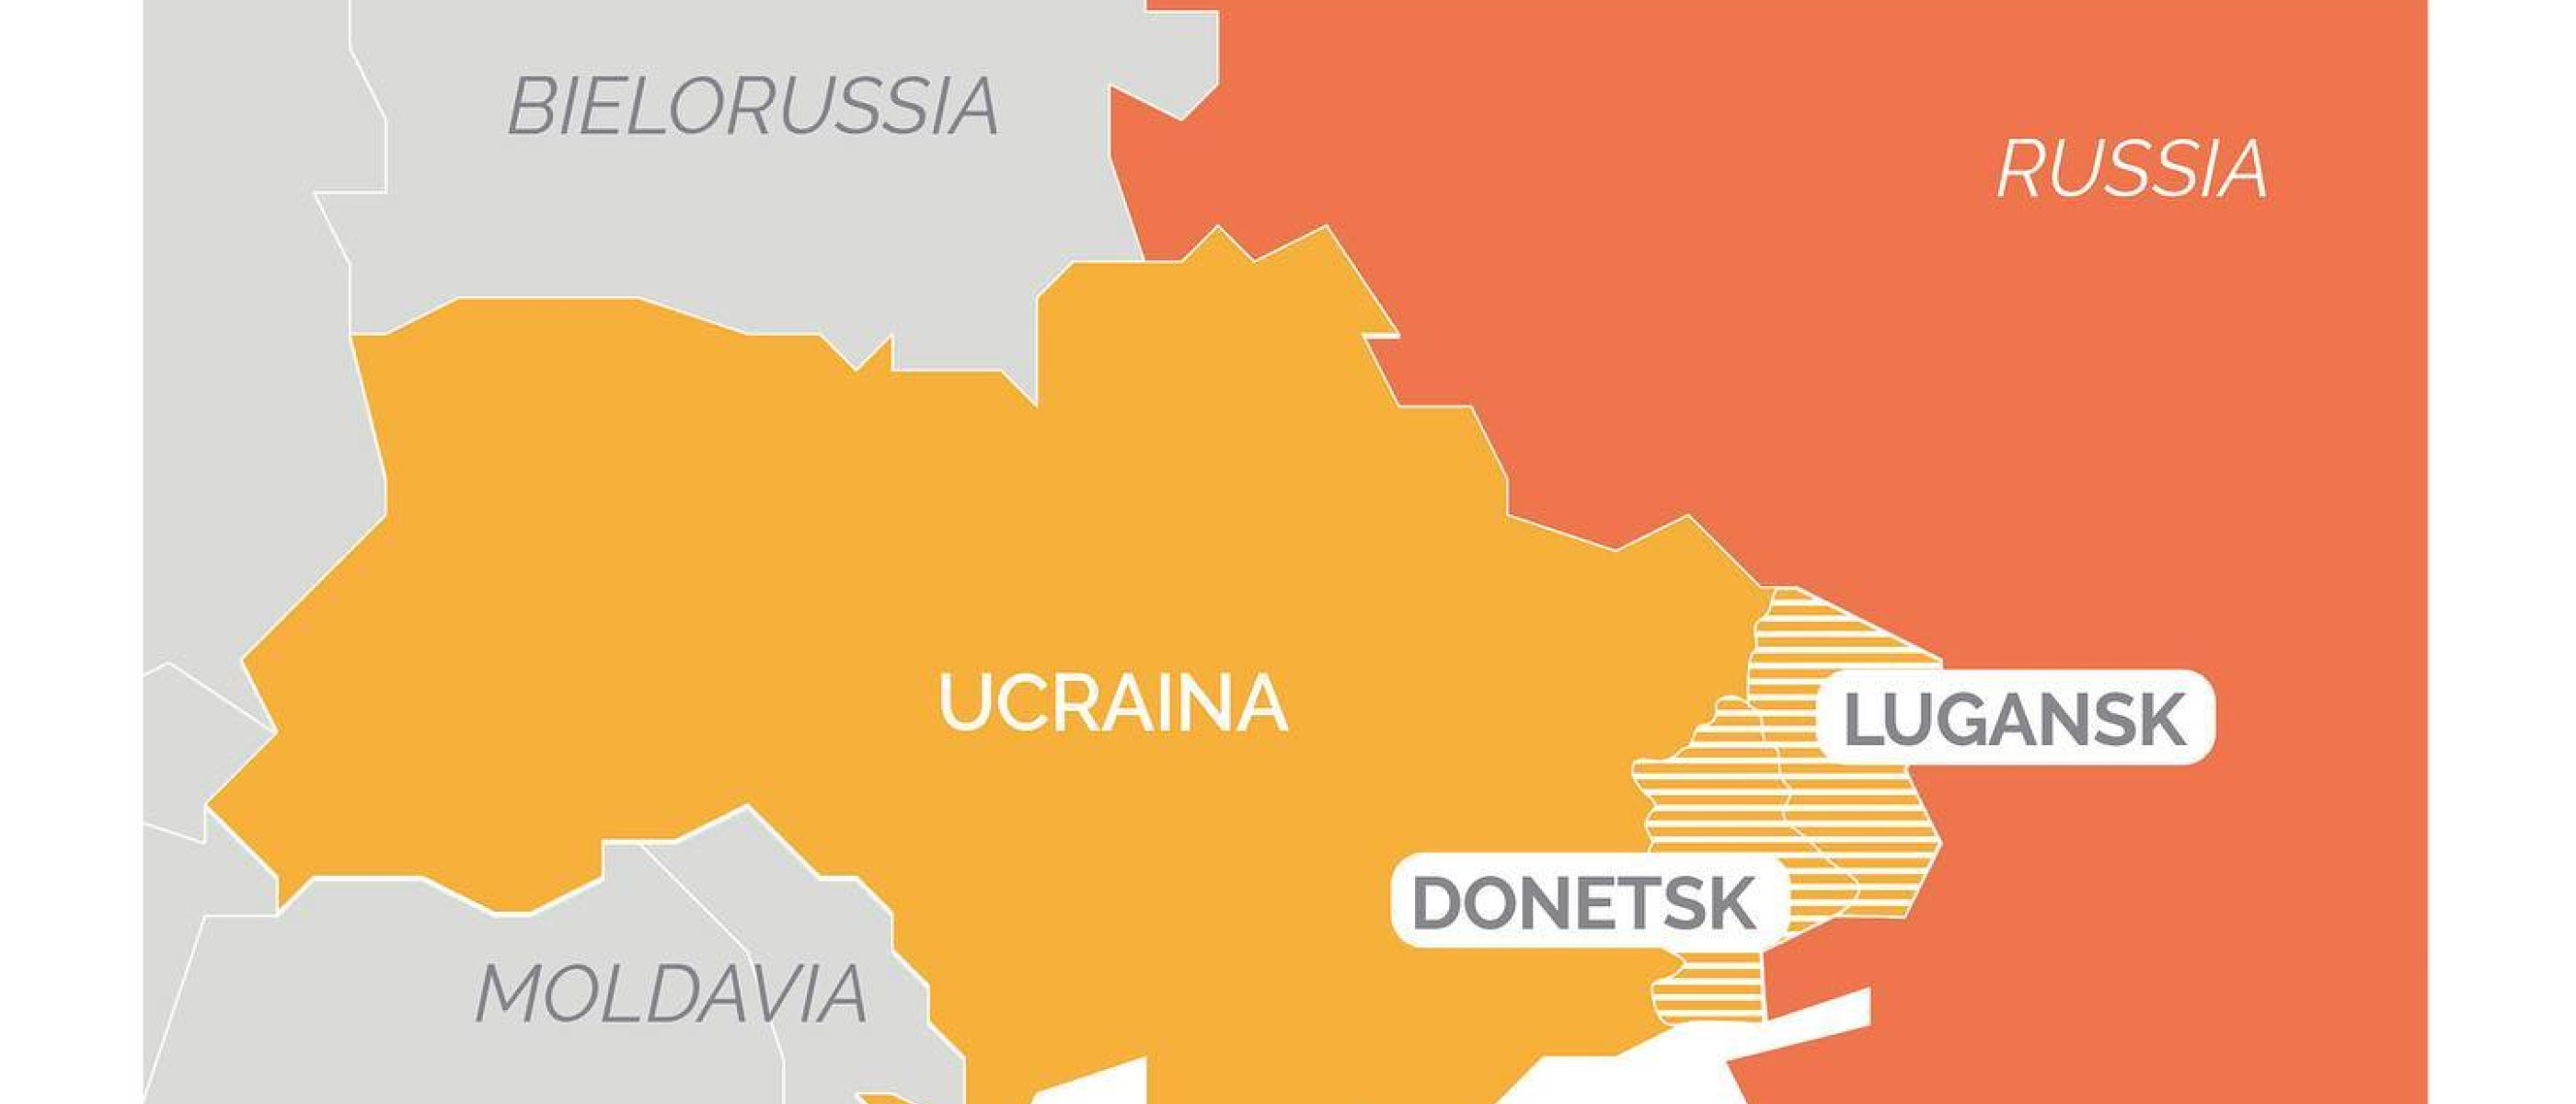
\includegraphics[width=0.75\textwidth]{images/map.jpg}
    \caption{Cartina geografica Russia, Ucraina e Donbass}
\end{figure}

% https://www.geopop.it/i-motivi-per-cui-la-Russia-di-putin-vuole-il-donbass-la-nuova-fase-della-guerra-in-ucraina/

% https://www.ispionline.it/it/pubblicazione/russia-ucraina-putin-riconosce-le-repubbliche-separatiste-del-donbass-33851

\pagebreak

\subsubsection{Le sanzioni nei confronti della Russia}

L'unione europea ha imposto alla Russia delle sanzioni per avvertirli del loro disaccordo nei confronti della guerra. L'obiettivo principale di queste sanzioni consiste nel ridurre la potenza economica della Russia, riducendo le possibilità di costruire armamenti bellici. Queste sanzioni hanno permesso di risparmiare molte vite. Questo perché in diversi casi la Russia ha dovuto ritirarsi dal combattimento a seguito della fine delle risorse a disposizione per combattere. Se non fossero state applicate le sanzioni questi soldati (sia Ucraini che Russi) sarebbero morti. Ci sono stati altri provvedimenti per punire coloro che dalla guerra avrebbero tratto dei vantaggi economici.

\subsubsection{Le conseguenze economiche ed energetiche per le altre nazioni}

La Russia ad oggi è uno dei più grandi fornitori di gas, petrolio e carbone per l'Europa. Fornisce il 40\% del suo petrolio / carbone e il 20\% del suo quantitativo di gas. Nelle altre nazioni il costo di tutti questi elementi è aumentato drasticamente proprio per il fatto che non hanno la possibilità di produrre tutta l'energia necessaria internamente. A causa delle sanzioni emanate nei confronti della Russia, è stato ridotto l'apporto di gas verso l'Europa dai condotti dei due gasdotti principali russi, nonché Nord Stream 1 e Nord Stream 2. Anche in Svizzera la situazione si è fatta abbastanza critica, la crisi del gas ha fatto aumentare drasticamente i prezzi fino a portare le persone a fare rifornimento subito per evitare di dover spendere molto di più in seguito. Le conseguenze si potrebbero vedere anche durante quest'inverno con dei possibili black-out programmati per limitare il consumo energetico.

\begin{figure}[h]
    \centering
    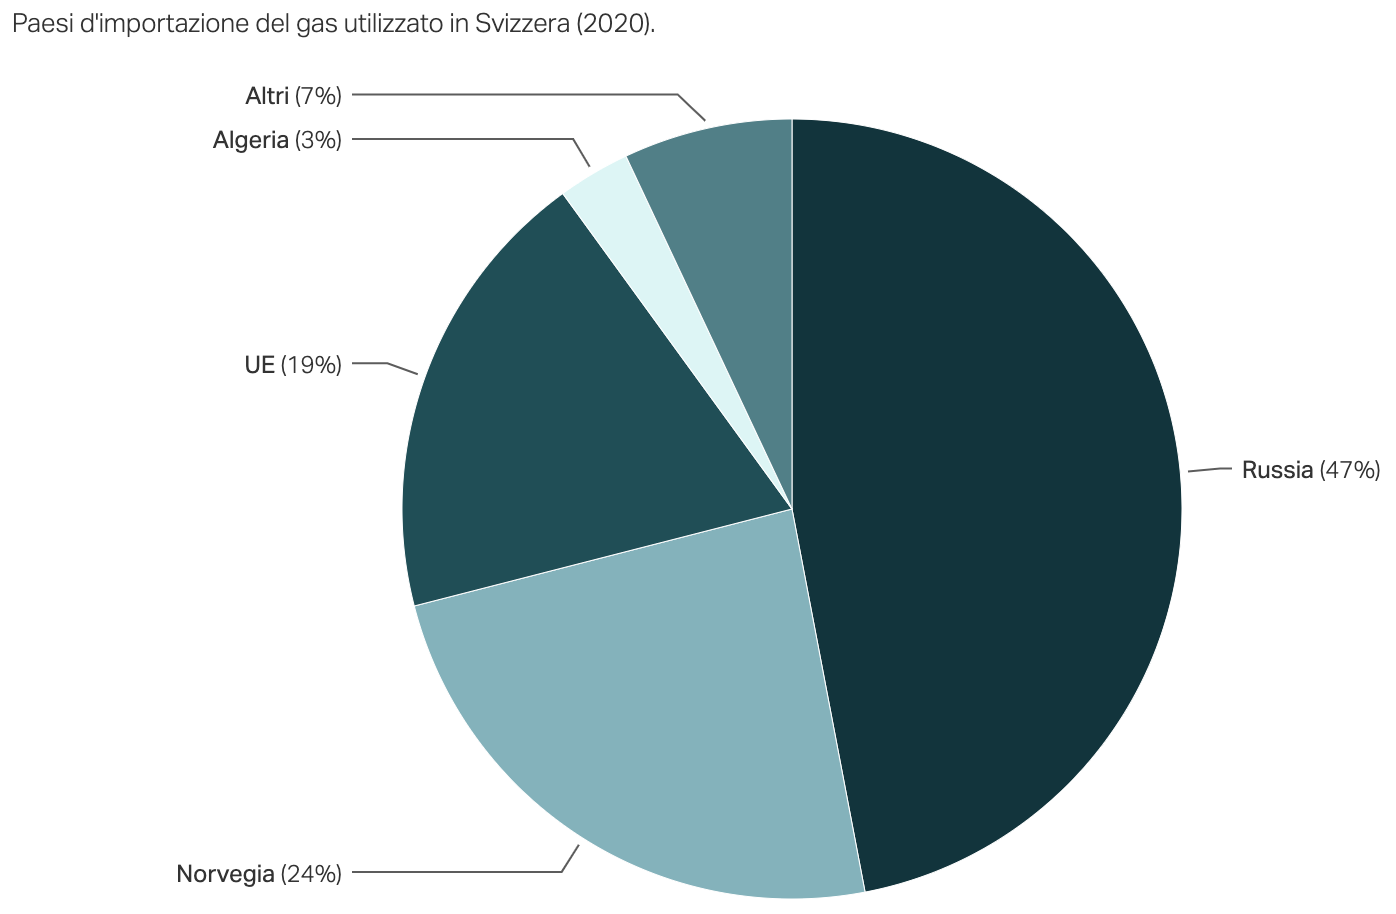
\includegraphics[width=0.75\textwidth]{images/grafico_provenienza_gas_svizzera.png}
    \caption{Grafico provenienza gas in Svizzera}
\end{figure}

%https://it.wikipedia.org/wiki/Nord_Stream%

%https://www.swissinfo.ch/ita/politica/guerra-ucraina-energia-gas-russia-svizzera/47460144

\pagebreak

\subsubsection{Il valore della vita dei soldati andati in guerra}

Per gli alti ufficiali dell'esercito russo, la vita dei loro soldati non ha alcuna importanza. Grazie ad una testimonianza trovata online si può vedere un ragazzo russo che spiega la situazione drammatica. Decine di soldati sono stati abbandonati dagli alti ranghi dell'esercito al freddo e con poco cibo e acqua (sufficiente per tre giorni). Questi soldati avevano creduto alle parole degli ufficiali che dicevano che sarebbero tornati a prenderli. Così non è stato. Questi soldati sono stati abbandonati a loro stessi. L'esercito russo usa queste persone come se fossero carne da macello, persone di poca importanza. Insomma la loro vita per gli ufficiali non conta nulla. Essi perdono la vita per la loro nazione ed è questo il ringraziamento che ottengono. Sono pronti a perdere la vita per una nazione per cui non contano nulla. L'unico altro motivo che c'è per il quale queste persone vanno a combattere è per difendere la propria famiglia e per garantirle un futuro più felice. \\ Molte delle persone che vanno a combattere sono persone con già famiglia. Un sondaggio fatto da Russian Field dichiara che la maggior parte delle persone che vanno in guerra sono soprattutto anziani e persone poco istruite. Questo sondaggio mostra come un giovane su due non concorda con l'aggressione russa. Nella fascia di età tra i 18 e i 29 anni il 41,1\% dichiara di essere favorevole all'aggressione, mentre il 49,9\% non lo è. La percentuale di persone favorevoli alla guerra aumenta nella fascia persone più anziane (circa 50-60 anni) con un tasso del 72,8\%. \\ Con questo si vuole dimostrare come i giovani tengano di più alla loro vita e alla pace, anche perché forse non hanno una famiglia a cui dover badare.

\pagebreak

\section{I mondiali del Qatar}

\subsection{La situazione politica}

Il sistema politico in Qatar è la monarchia assoluta. Tutto il potere è detenuto dalla famiglia al-Thani. Attualmente Tamim bin Hamad al-Thani ha 42 anni ed è sposato con Noora bint Hathal Al Dosar.

% https://www.ilpost.it/2022/11/18/qatar/

\begin{figure}[h]
    \centering
    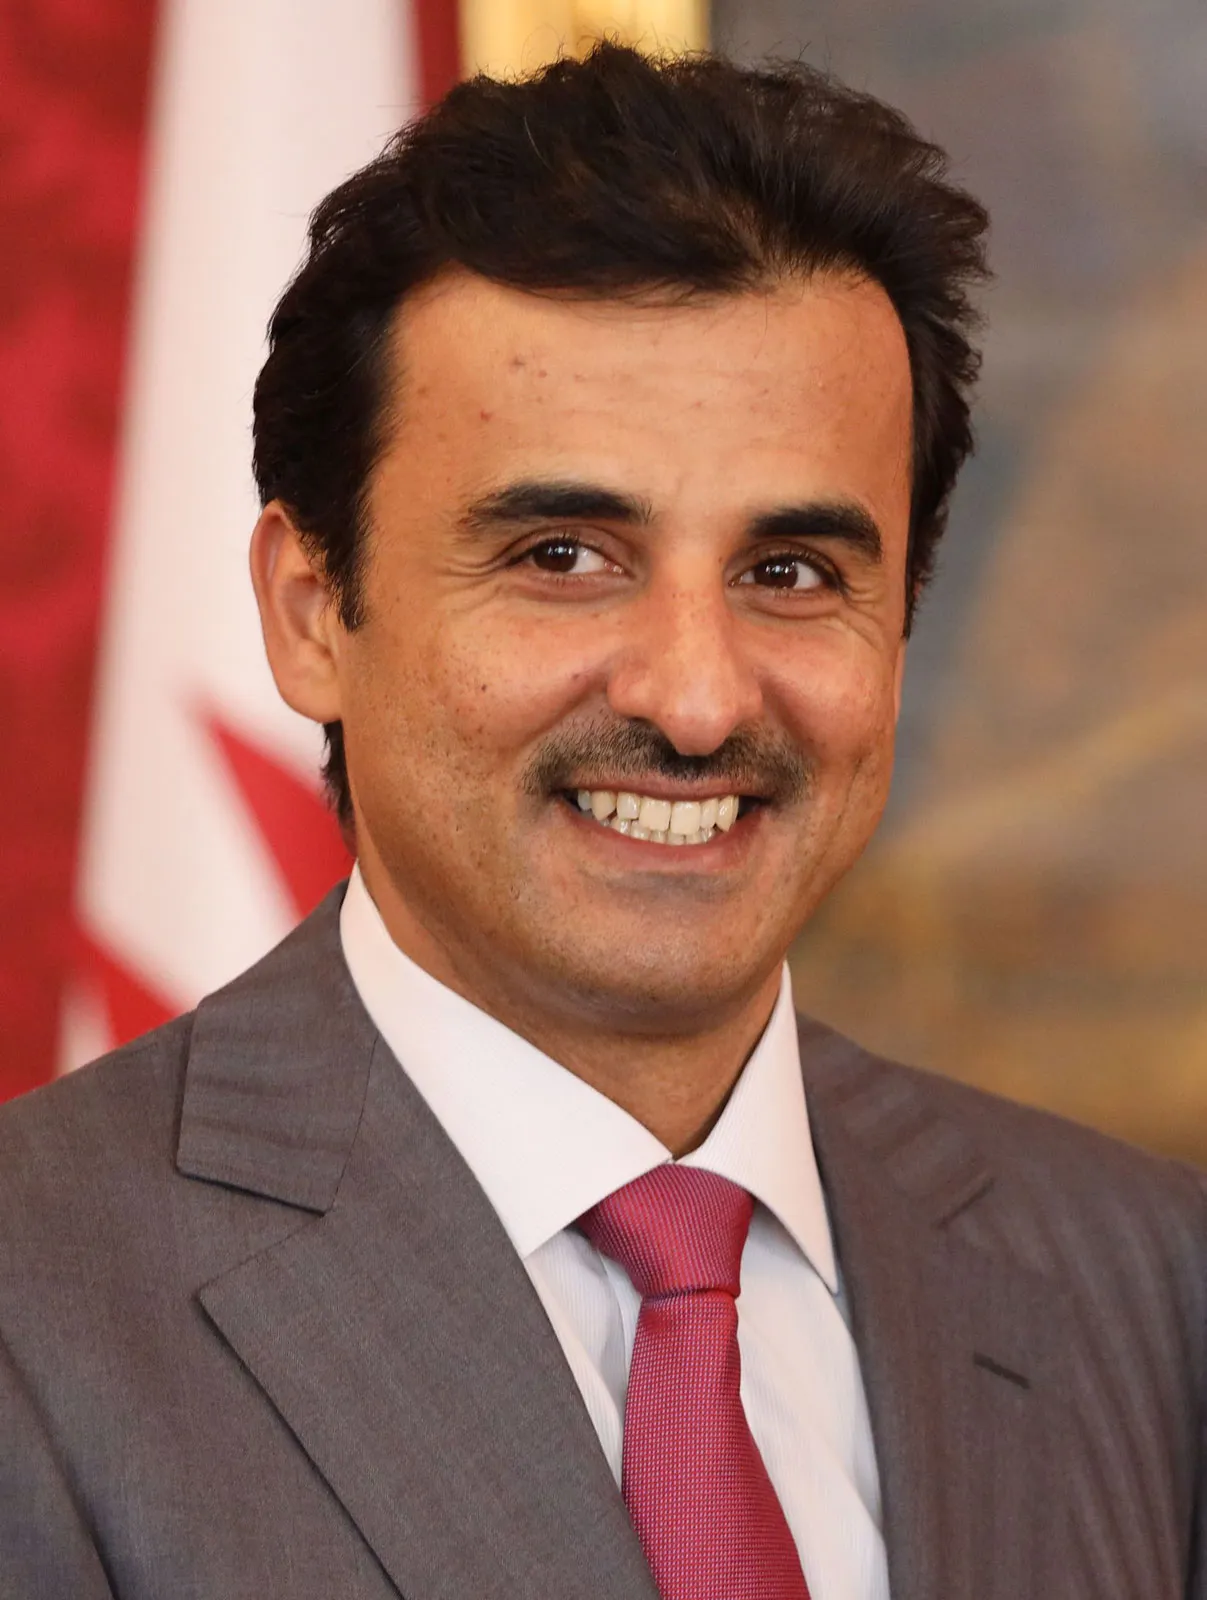
\includegraphics[width=0.5\textwidth]{images/sheikh.png}
    \caption{Sceicco Tamim bin Hamad al-Thani}
\end{figure}

% https://en.wikipedia.org/wiki/Politics_of_Qatar

% https://www.britannica.com/biography/Sheikh-Tamim-ibn-Hamad-Al-Thani

\subsection{Le sanzioni}

In Qatar ci sono delle sanzioni molto pesanti. È ancora in vigore la pena di morte. Inoltre, la lapidazione è una punizione legale in Qatar. Il fatto di non voler più credere nella propria religione è soggetto alla pena di morte. I bestemmiatori sono punibili con una sanzione fino a 7 anni di detenzione e il fatto di cambiar religione o partito politico è punibile con una sanzione fino a 10 anni di detenzione. Inoltre, l'omosessualità è punibile con la pena di morte. Per chi commette adulterio verrà inflitta una sanzione di 100 frustate.

\pagebreak

\subsection{Il consumo di alcol}

In Qatar è consentito il consumo di bevande alcoliche. Le persone non musulmane possono bere le bevande alcoliche. I musulmani no. Se vengono scoperti a bere alcolici ricevono una sanzione che va dalla fustigazione alla deportazione. La fustigazione consiste in un massimo di 100 frustate. Di conseguenza il vero motivo della limitazione del consumo di alcolici è dovuto ad un motivo religioso e non da attribuirsi alla precauzione della salute dei cittadini. Nello stadio del mondiale è consentito bere solo birra ma soprattutto di una sola marca. Per la Budweiser, azienda di birra sponsor dei mondiali con 75 milioni di dollari investiti, non è stato consentito allestire i suoi stand. A Budweiser è stato permesso di vendere la sua birra esclusivamente ai Vip nelle aree Hospitality in tribuna. Tutto questo è dovuto sempre al motivo religioso. I costi all'interno dello stadio per bere sono estremamente alti. Si parla di 14 euro per mezzo litro di Coca Cola. Prima dei mondiali il consumo di birra (non altri alcolici) era permesso solamente all'interno di hotel di lusso con dei prezzi estremamente alti. 

\subsection{Lo sfruttamento violento dei lavoratori}

Lo sfruttamento è di vario tipo. Va dallo sfruttamento fisico allo sfruttamento  economico. Lo sfruttamento fisico consiste nel fare lavorare le persone più tempo di quello che potrebbero o quello che dovrebbero lavorare. Lo sfruttamento economico consiste nel fare avere un salario ai lavoratori molto basso, con molte spese a carico del lavoratore. I lavoratori vengono pagati molto poco. La maggior parte di questi lavoratori sono migranti che arrivano dal Bangladesh e Nepal. Vanno in Qatar perché possono guadagnare di più rispetto al loro paese. Per poter lavorare in Qatar ti serve un visto ed un lavoro. Devi pagare sia il visto che il lavoro. Queste persone devono pagare da 1000 a 4000 dollari per ottenere visto e lavoro. La maggior parte di loro non possiede questi soldi, quindi deve fare un debito. A questo punto possono cominciare a lavorare. Il guadagno medio è di 275 dollari. Per poter ripagare questo debito i lavoratori devono lavorare per più di un anno. Dopo aver ripagato il debito possono cominciare a guadagnare per vivere, anche se guadagnano molto poco.

%https://www.repubblica.it/sport/calcio/esteri/2022/04/01/news/lavoratori_sfruttati_morti_mondiali_qatar_stadi-343708561/

\pagebreak

\subsection{La risposta della FIFA riguardo ai mondiali}

La FIFA, ovvero la federazione internazionale delle società calcistiche si impegna nella salvaguardia degli operai. Amnesty International ha comunicato alla FIFA di dover risarcire i lavoratori per un totale di 440 millioni di dollari. \\ Il governo del Qatar ha affermato che il numero di decessi è proporzinale alla forza lavoro migrante e che i dati riportano anche le morti naturali. \cite{cosaPensaFIFA} \\ Secondo noi queste affermazioni sono estreme, perché non è normale calcolare la morte dei lavoratori esteri come se fosse qualcosa di normale. L'unica azione buona che il Qatar ha fatto nei confronti dei suoi dipendenti è stata rendere l'assistenza sanitaria gratuita per i lavoratori stranieri. \\ Questo ci porta a credere che nonostante il Qatar prenda con leggerezza la morte degli operai, un minimo gli importa della vita di queste persone. La FIFA afferma di essere profondamente dispiaciuta per tutte quelle morti.

\begin{figure}[h]
    \centering
    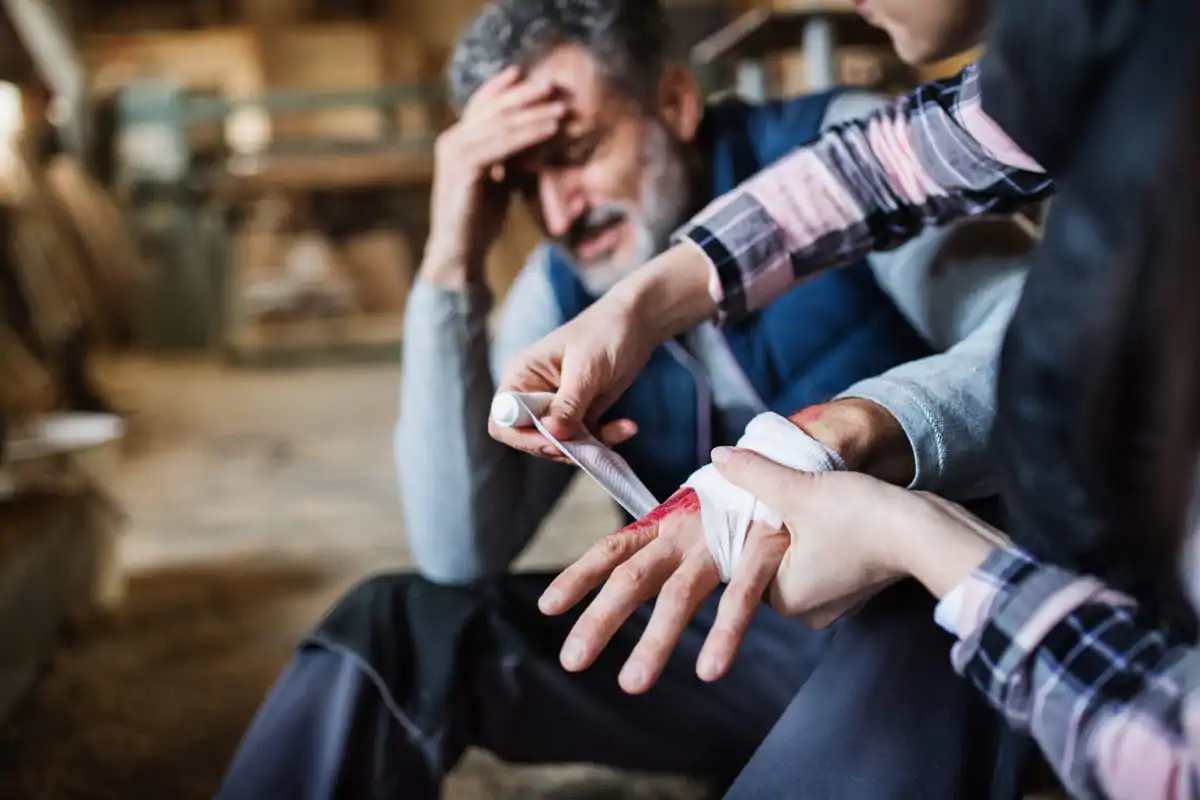
\includegraphics[width=0.65\textwidth]{images/mondiali_qatar_2022_lavoratori.png}
    \caption{Lavoratore ferito mentre viene medicato}
\end{figure}

% https://www.abilitychannel.tv/mondiali-qatar-2022-lavoratori-migranti/#Mondiali_Qatar_2022_e_lavoratori_migranti_come_funziona_il_sistema

\pagebreak

\subsection{Il costo della vita in Svizzera}

In questo grafico si può notare che la maggior parte dei beni hanno un prezzo più elevato in svizzera. Fanno eccezione gli alcolici. Questi ultimi costano di più in Qatar perché la religione nazionale permette il consumo di alcolici solo in determinate circostanze, quindi vengono venduti meno.

\begin{figure}[h]
    \centering
    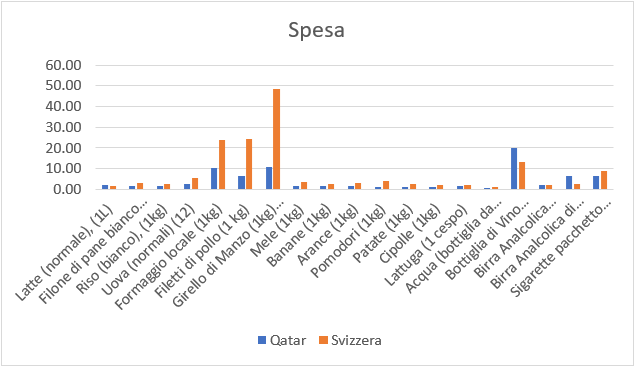
\includegraphics[width=0.8\textwidth]{images/spesa.png}
    \caption{Differenza costo spesa Qatar vs Svizzera}
\end{figure}

Nel grafico dei ristoranti si ripresenta la situazione precedente, quindi le bevande alcoliche ad un prezzo più elevato di quello svizzero.

\begin{figure}[h]
    \centering
    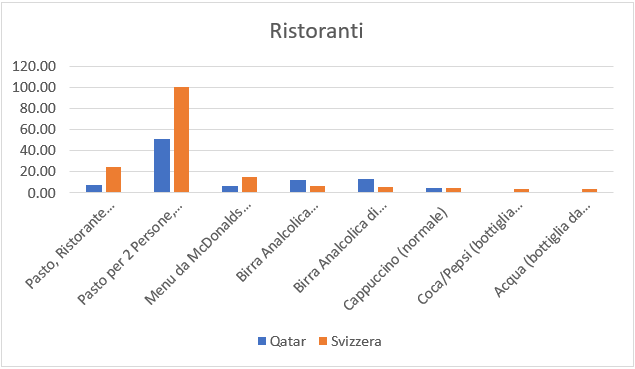
\includegraphics[width=0.8\textwidth]{images/ristorante.png}
    \caption{Differenza costo ristoranti Qatar vs Svizzera}
\end{figure}

\pagebreak

\begin{figure}[h]
    \centering
    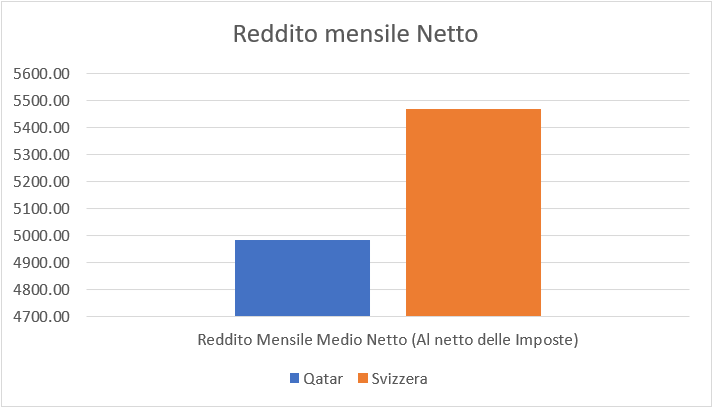
\includegraphics[width=0.8\textwidth]{images/reddito.png}
    \caption{Differenza costo spesa Qatar vs Svizzera}
\end{figure}

\begin{figure}[h]
    \centering
    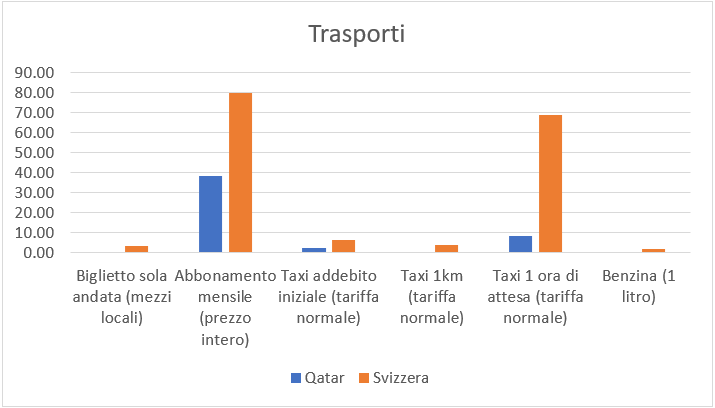
\includegraphics[width=0.8\textwidth]{images/trasporti.png}
    \caption{Differenza costo trasporti Qatar vs Svizzera}
\end{figure}

\pagebreak

\begin{figure}[h]
    \centering
    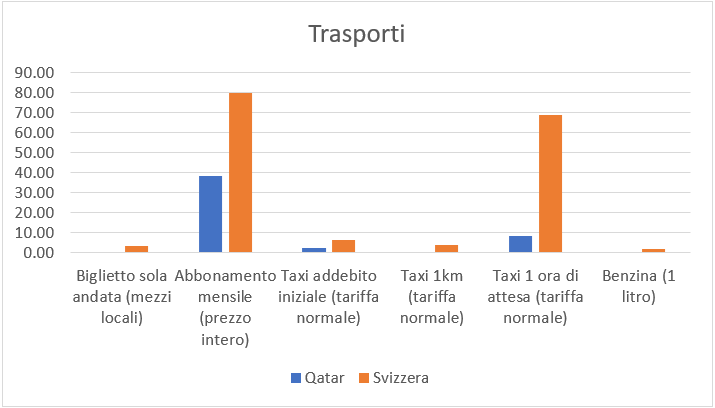
\includegraphics[width=0.8\textwidth]{images/svago.png}
    \caption{Differenza costo svago Qatar vs Svizzera}
\end{figure}

\begin{figure}[h]
    \centering
    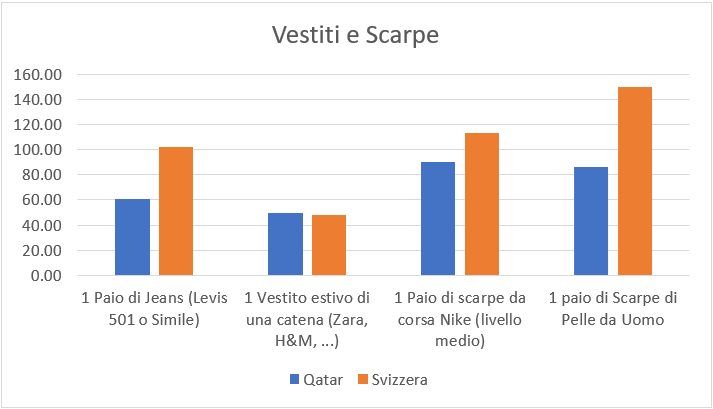
\includegraphics[width=0.8\textwidth]{images/vestiti.png}
    \caption{Differenza costo vestiario Qatar vs Svizzera}
\end{figure}

\pagebreak

\begin{figure}[h]
    \centering
    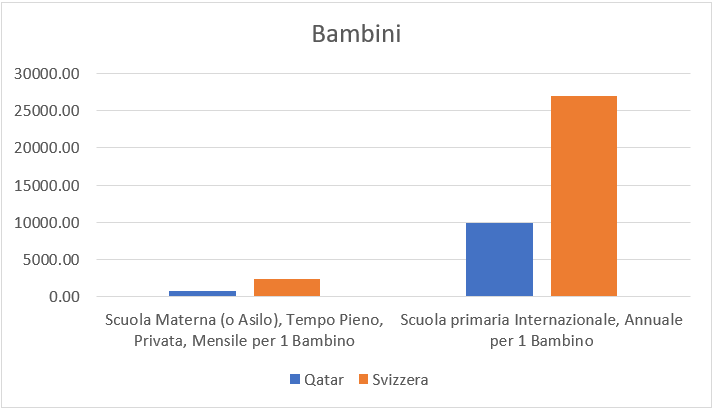
\includegraphics[width=0.8\textwidth]{images/bambini.png}
    \caption{Differenza costo bambini Qatar vs Svizzera}
\end{figure}

\begin{figure}[h]
    \centering
    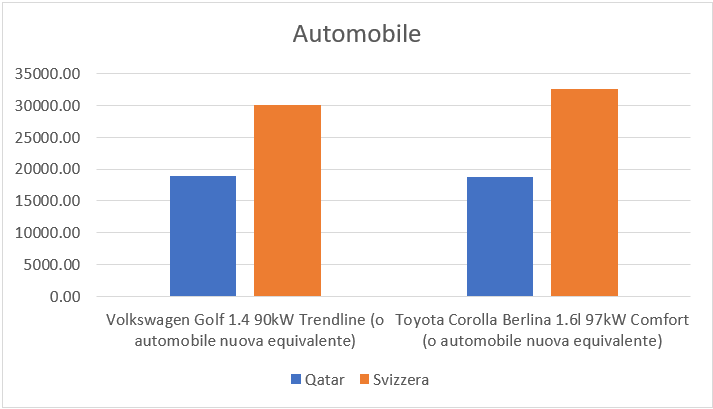
\includegraphics[width=0.8\textwidth]{images/automobile.png}
    \caption{Differenza costo automobile Qatar vs Svizzera}
\end{figure}

\pagebreak

\begin{figure}[h]
    \centering
    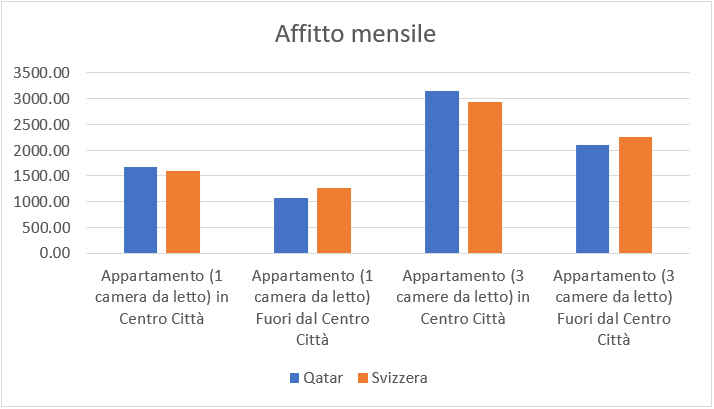
\includegraphics[width=0.8\textwidth]{images/affitto.png}
    \caption{Differenza costo affitto Qatar vs Svizzera}
\end{figure}

\begin{figure}[h]
    \centering
    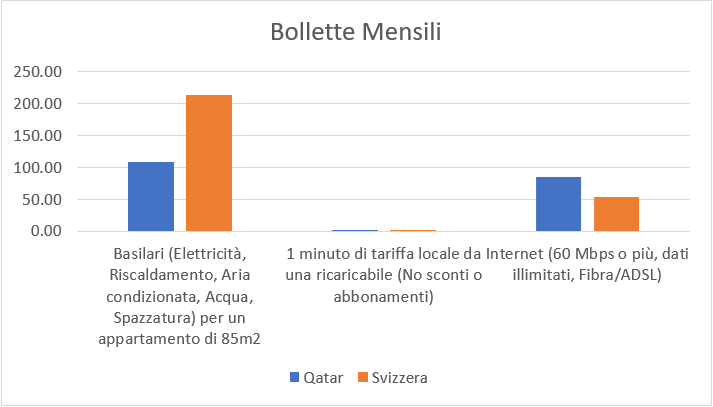
\includegraphics[width=0.8\textwidth]{images/bollette.png}
    \caption{Differenza costo bollette Qatar vs Svizzera}
\end{figure}

\pagebreak

\begin{figure}[h]
    \centering
    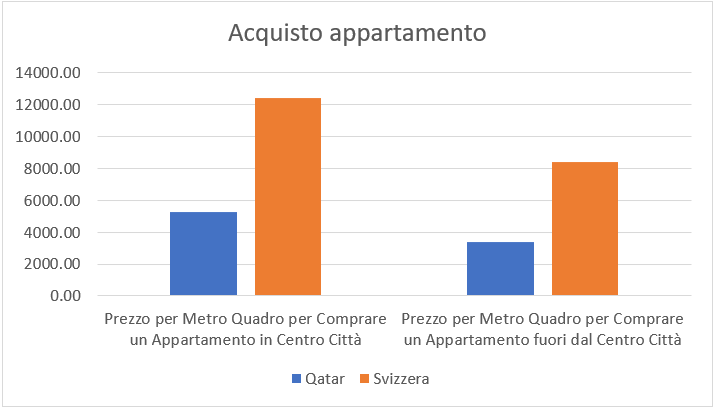
\includegraphics[width=0.8\textwidth]{images/appartamento.png}
    \caption{Differenza costo acquisto appartamento Qatar vs Svizzera}
\end{figure}

\begin{figure}[h]
    \centering
    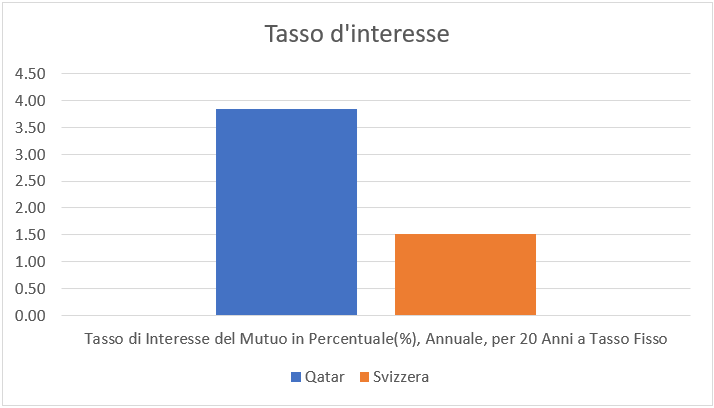
\includegraphics[width=0.8\textwidth]{images/tassointeresse.png}
    \caption{Differenza tasso d'interesse Qatar vs Svizzera}
\end{figure}

% https://it.numbeo.com/costo-della-vita/nazione/Qatar?displayCurrency=CHF
% https://it.numbeo.com/costo-della-vita/nazione/Svizzera

\pagebreak

\section{Conclusioni}

\subsection{Samuel Banfi}

Nel corso di questo progetto siamo riusciti a completare i nostri obiettivi di percorso. Tra i quali troviamo la dimostrazione che alla Russia non interessa la vita dei suoi cittadini. Invece siamo riusciti a dimostrare come il Qatar abbia fatto sacrificare la vita a moltissimi lavoratori solamente per costruire uno stadio. Personalmente ho riscontrato un po' di difficoltà a trovare le informazioni riguardo alla condizioni di vita dei soldati al fronte. Mi è stato anche difficile trovare le informazioni riguardo ai giornalisti uccisi. Questo perché trovavo dei siti dove le informazioni venivano confermate e altri siti dove queste informazioni venivano smentite. Sono dell'idea che fare questo progetto a gruppi mi ha aiutato a capire la difficoltà di spartirsi i lavori. In alcuni casi ci siamo ritrovati a lavorare sullo stesso capitolo. Personalmente sono soddisfatto del risultato ottenuto, anche perché un lavoro del genere non è qualcosa che si fa tutti i giorni. Inoltre mi ha fatto crescere mentalmente scoprendo quella succede dietro le quinte di un mondiale. In televisione viene mostrata solo la parte bella dei mondiali ma non vengono mai mostrati gli orrori che succedono durante la costruzione di uno stadio, in questi paesi dove la possibilità di crescita personale è molto limitata.

\subsection{Dennis Donofrio}

Mi è piaciuto come siamo riusciti a lavorare durante questo progetto. All'inizio avevamo un indice un po' ambizioso e strada facendo lo abbiamo dovuto stringere. Mi sono occupato principalmente della parte del Qatar. Questo mi ha fatto riflettere. È incredibile pensare che in questo momento io sono seduto su una sedia a scrivere al computer mentre qualcuno sta lavorando e soffrendo in Qatar per poter sopravvivere. Ho fatto un po' fatica a reperire delle informazioni, probabilmente per la mia inesperienza in ricerche in questo campo. Infatti questo progetto mi ha aiutato a migliorare la mia tecnica di ricerca. Alla fine posso dire che sono soddisfatto di come è uscito questo progetto. Non ne avevo mai fatto nessuno di questo genere.

\pagebreak

\section{Bibliografia}

\section{Sitografia}

\nocite{*}
\printbibliography[type=online, heading=subbibliography] 	

\end{document}